\section{Design und Development}
Gemäss Peffers werden in dieser Phase das eigentliche Artefakt entwickelt. Hierzu gehört die Definition der Anforderungen sowie die eigentliche Entwicklung des Artefakts ~\citep[S. 55]{peffers}. Die Anforderungen wurden im Rahmen dieser Arbeit bereits im Kapitel \ref{ch:definition_of_objectives} erhoben, da sich die Anforderungserhebung gut mit der Auswertung des Untersuchungsinstrumentes kombinieren lässt. Als Teil dieses Kapitels wird daher primär auf die eigentliche Entwicklung des Artefaktes eingegangen. Beim Entwickeln des Artefakts hat sich der Autor für das Erstellen einer \textbf{In-House} Lösung entschieden, da somit die Flexibilität in Bezug auf Datenvisualisierungen und Funktionalitäten sichergestellt werden kann (siehe Kapitel \ref{ch:theory_in_house_solutions}).

Die Entwicklung des Artefakts wird sich hierbei auf drei Teilbereiche beschränken. Zu Beginn wird auf die Auswahl der Datenquelle eingegangen. Anschliessend folgt 

\subsection{Auswahl der Datenquelle}
In einem ersten Schritt wurden die Art der Daten sowie die eigentliche Datenquelle identifiziert. Bei den darzustellenden Daten handelt es sich hierbei um \textbf{quantitative} Daten (siehe Kapitel \ref{ch:data_selection}). Als Datenquelle wurden die gleichen Daten verwendet, wie sie auch vom Corona Dashboard der Schweiz (siehe Kapitel \ref{ch:creation_of_interview_guide}) verwendet werden. Der Autor ist sich an dieser Stelle bewusst, dass sich die hier aufgeführten Daten nur auf die Schweiz beziehen. Da jedoch die Filterung nach Regionen als Anforderung definiert wurde und im Fall der gesamten Welt viele Anwendungsfälle zu berücksichtigen sind, wurde diese Entscheidung bewusst getroffen. Die Daten werden hierbei in unterschiedlichen Dateiformaten vom \gls{foph} im Rahmen des opendata.swiss Projektes zur Verfügung gestellt (siehe Abbildung \ref{fig:covid19_open_data}). Da es anhand der definierten Anforderungen um die Darstellung von Corona Todesfallzahlen sowie Spitalauslastungen geht, wurden entsprechend die Datensätze COVID19Death\_geoRegion.csv sowie COVID19HospCapacity\_geoRegion.csv verwendet.

\begin{figure}[h]
    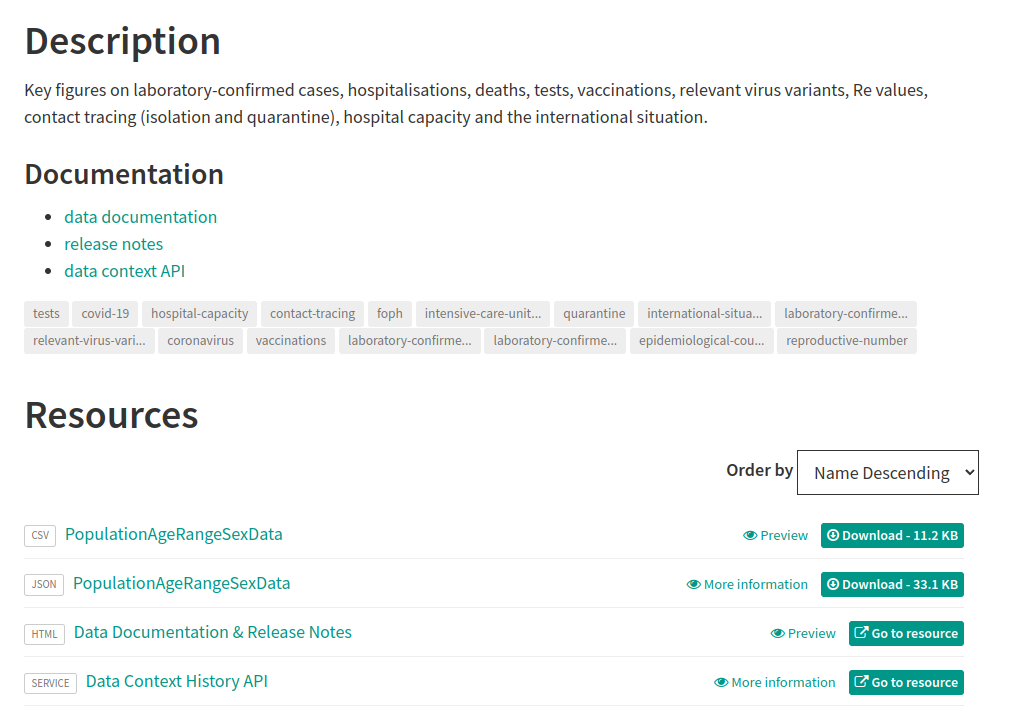
\includegraphics[width=12cm]{images/covid_data_set.png}
    \centering
    \caption{Covid Datensätze von opendata.swiss ~\citep{covid19_open_data}}
    \label{fig:covid19_open_data}
\end{figure}

\subsection{Implementierung des Frontend}
TODO

\subsection{Implementierung des Backend}
TODO
